\chapter{Supplementary Material for Contribution 3 (RQ3)}\label{app:rq3}

The content of this appendix is based on \citeauthor{GOLAB2026SpatialTruck} (\citeyear{GOLAB2026SpatialTruck}).

\section{Extended nomenclature}\label{app:rq3_nomenclature}

Table~\ref{tab:nomenclature_rq3_app} lists the extended nomenclature for the long-distance freight transport decarbonization model described in Section~\ref{sec:rq3_extension}. Compared to the core model nomenclature (Table~\ref{tab:nomenclature_main}), consumer groups ($u$) and vehicle types ($v$) are dropped, as a single vehicle type (trucks) is considered. The technology index $t$ directly distinguishes ICEV and BET for road transport and rail. A mode index $m \in \mathcal{M}$ is introduced for road and rail transport. The flow variable $f_{yrmtg}$ represents annual freight tonnage rather than person-trips, and the payload $W_{tg}$ represents tonnes per vehicle rather than persons per vehicle.

\begin{scriptsize}
\begin{longtable}{llll}
\caption{Extended nomenclature for the long-distance freight transport decarbonization model (RQ3).}
\label{tab:nomenclature_rq3_app}\\
\hline
Sets and indices & Description & & \\ \hline
\endfirsthead
\endhead
\hline
\endfoot
\endlastfoot
$y \in \mathcal{Y}$ & year & & \\
$r \in \mathcal{R}$ & route between origin-destination (OD) pair & & \\
$t \in \mathcal{T}$ & \begin{tabular}[t]{@{}l@{}}drivetrain technology\\(ICEV, BET for road; rail)\end{tabular} & & \\
$g \in \mathcal{G}$ & year that vehicle was introduced to market & & \\
$m \in \mathcal{M}$ & transport mode (road, rail) & & \\
$e \in \mathcal{E}$ & geographic location (NUTS-2 region) & & \\
$\mathbf{E}_r$ & ordered set of geographic locations along route $r$ & & \\
$e_{r,i}$ & $i$-th geographic location along route $r$ & & \\
$l \in \mathcal{L}$ & types of fueling infrastructure (by capacity) & & \\
$\mathcal{Y}^{\mathrm{exp}}$ & set of years of investment decisions & & \\
$\mathcal{Y}^{\mathrm{exp}}_y$ & subset of investment years up to year $y$ & & \\
$\mathcal{T}_m$ & technologies available for mode $m$ & & \\
$\mathcal{T}^{\mathrm{road}}$ & road technologies (ICEV, BET) & & \\
$\mathcal{T}^{\mathrm{rail}}$ & rail technology & & \\
$\mathcal{T}^{\mathrm{BET}}$ & battery-electric truck technology & & \\
$\mathcal{T}^{\mathrm{ICEV}}$ & internal combustion engine technology & & \\
$\mathcal{R}_{e}$ & set of routes that go through location $e$ & & \\
$\mathcal{L}_{t}$ & \begin{tabular}[t]{@{}l@{}}types of fueling infrastructure\\by drivetrain technology\end{tabular} & & \\
$\mathcal{E}_{r}$ & \begin{tabular}[t]{@{}l@{}}set of geographic locations\\along route $r$\end{tabular} & & \\
\\\hline
Decision variables & Description & Unit & Domain \\ \hline
$f_{yrmtg}$ & freight flow by mode & t/a & $[0,\infty[$ \\
$h_{yrtg}$ & number of vehicles & -- & $[0, \infty[$ \\
$h^{+}_{yrtg}$ & newly purchased vehicles & -- & $[0,\infty[$ \\
$h^{-}_{yrtg}$ & \begin{tabular}[t]{@{}l@{}}number of vehicles leaving\\the vehicle stock\end{tabular} & -- & $[0, \infty[$ \\
$s_{yrtgle}$ & energy fueled & kWh & $[0, \infty[$ \\
$soc_{yrtge}$ & \begin{tabular}[t]{@{}l@{}}fleet-aggregate state of charge\\at location $e$\end{tabular} & kWh & $[0, \infty[$ \\
$travel\_time_{yrtge}$ & \begin{tabular}[t]{@{}l@{}}fleet-aggregate accumulated travel\\time at location $e$\end{tabular} & h & $[0, \infty[$ \\
$break\_time^{+}_{yrtge}$ & \begin{tabular}[t]{@{}l@{}}time on mandatory break not\\used for charging\end{tabular} & h & $[0, \infty[$ \\
$q^{+, \mathrm{charg\_infr}}_{ytle}$ & added charging infrastructure & kW & $[0, \infty[$ \\
$h^{\mathrm{exist}}_{yrtg}$ & \begin{tabular}[t]{@{}l@{}}vehicles carried over from\\previous period\end{tabular} & -- & $[0, \infty[$ \\
\\\hline
Parameters & Description & Unit & Domain \\ \hline
$y_0$ & initial (base) year & -- & -- \\
$F_{yr}$ & exogenous freight demand & t/a & $[0, \infty[$ \\
$F^{\mathrm{rail}}_y$ & total rail freight flow in year $y$ & t$\cdot$km & $[0, \infty[$ \\
$F^{\mathrm{total}}_y$ & total freight flow in year $y$ & t$\cdot$km & $[0, \infty[$ \\
$D^{\mathrm{spec}}_{tg}$ & specific energy consumption & kWh/km & $[0, \infty[$ \\
$W_{tg}$ & payload capacity (tonnes per vehicle) & t & $[0, \infty[$ \\
$L_r$ & length of route $r$ & km & $[0, \infty[$ \\
$L_{e_{(i-1,i)}}$ & \begin{tabular}[t]{@{}l@{}}distance between consecutive\\geographic locations\end{tabular} & km & $[0, \infty[$ \\
$L^{\mathrm{annual}}_{tg}$ & annual mileage & km & $[0, \infty[$ \\
$\mathrm{Cap}^{\mathrm{tank}}_{tg}$ & tank capacity & kWh & $[0, \infty[$ \\
$Q^{\mathrm{batt}}_{tg}$ & battery capacity & kWh & $[0, \infty[$ \\
$\hat{P}_{tg}$ & charging power & kW & $[0, \infty[$ \\
$SOC^{\mathrm{init}}$ & \begin{tabular}[t]{@{}l@{}}initial state of charge\\(fraction of battery capacity)\end{tabular} & -- & $[0, 1]$ \\
$SOC^{\mathrm{final}}$ & \begin{tabular}[t]{@{}l@{}}minimum final state of charge\\(fraction of battery capacity)\end{tabular} & -- & $[0, 1]$ \\
$\mathrm{SOC}^{+,\mathrm{charging}}$ & usable battery capacity for charging & -- & $[0, 1]$ \\
$speed$ & average driving speed (road) & km/h & $[0, \infty[$ \\
$TravelTime^{\mathrm{min}}_{e_{r,j}}$ & \begin{tabular}[t]{@{}l@{}}minimum cumulative travel time\\at node $j$ along route $r$\end{tabular} & h & $[0, \infty[$ \\
$\bar{\alpha}^{\mathrm{mode}}$ & maximum corridor-wide rail share & -- & $[0, 1]$ \\
$\alpha_f,\; \beta_f$ & \begin{tabular}[t]{@{}l@{}}rate-of-change parameters\\for modal shift\end{tabular} & -- & $[0, \infty[$ \\
$C^{\mathrm{CAPEX}}_{ytg}$ & expenditure costs for vehicles & \euro & $[0, \infty[$ \\
$C^{\mathrm{O\&M, veh}}_{ytg}$ & \begin{tabular}[t]{@{}l@{}}vehicle maintenance and\\repair costs\end{tabular} & \euro/a & $[0, \infty[$ \\
$C^{\mathrm{CAPEX, infr}}_{ytl}$ & \begin{tabular}[t]{@{}l@{}}capital expenditure for\\charging infrastructure\end{tabular} & \euro/kW & $[0, \infty[$ \\
$C^{\mathrm{O\&M, infr}}_{ytl}$ & \begin{tabular}[t]{@{}l@{}}operation and maintenance cost\\for charging infrastructure\end{tabular} & \euro/kW/a & $[0, \infty[$ \\
$c^{\mathrm{fuel}}_{ytle}$ & \begin{tabular}[t]{@{}l@{}}fuel or electricity cost\\at location $e$\end{tabular} & \euro/kWh & $[0, \infty[$ \\
$c^{\mathrm{grid}}_{e}$ & \begin{tabular}[t]{@{}l@{}}annual grid charge\\at location $e$\end{tabular} & \euro/kW/a & $[0, \infty[$ \\
$\mathrm{VoT}$ & value of time (freight) & \euro/h & $[0, \infty[$ \\
$\gamma_t$ & \begin{tabular}[t]{@{}l@{}}utilization factor (ratio of average\\to peak power demand)\end{tabular} & -- & $[0, 1]$ \\
$\delta$ & discount rate & -- & $[0, 1]$ \\
$\Delta y$ & \begin{tabular}[t]{@{}l@{}}time step between consecutive\\modeled periods\end{tabular} & a & $[0, \infty[$ \\
$\Lambda_{tg}$ & maximum vehicle lifetime & a & $[0, \infty[$ \\
$H^{\mathrm{init}}_{rtg}$ & initial vehicle stock & -- & $[0, \infty[$ \\
$Q^{\mathrm{charg\_infr}}_{tle}$ & initial charging infrastructure & kW & $[0, \infty[$ \\
$\hat{Q}^{\mathrm{charg\_infr}}_{tle}$ & \begin{tabular}[t]{@{}l@{}}upper limit for charging\\infrastructure capacity\end{tabular} & kW & $[0, \infty[$ \\
$\alpha^h,\; \beta^h$ & \begin{tabular}[t]{@{}l@{}}maximum stock transition\\rate parameters\end{tabular} & -- & $[0, \infty[$ \\
$\rho$ & \begin{tabular}[t]{@{}l@{}}maximum infrastructure\\growth rate per period\end{tabular} & -- & $[0, \infty[$ \\
$\tau_t(y)$ & \begin{tabular}[t]{@{}l@{}}technology-specific toll rate\end{tabular} & \euro/km & $[0, \infty[$ \\
$\overline{q}^{\mathrm{init}}$ & \begin{tabular}[t]{@{}l@{}}maximum new infrastructure investment\\in the initial period\end{tabular} & kW & $[0, \infty[$ \\
$c^{\mathrm{rail}}$ & levelized rail transport cost & \euro/tkm & $[0, \infty[$ \\
$c^{\mathrm{terminal}}$ & rail terminal handling cost & \euro/t & $[0, \infty[$ \\
\hline
\end{longtable}
\end{scriptsize}

\section{Extended mathematical formulation}\label{app:rq3_math}

This section provides the complete set of constraints of the long-distance freight transport decarbonization model. Constraints that are also presented with detailed explanations in Section~\ref{sec:rq3_extension} are included here for reference. Compared to the RQ2 formulation (Appendix~\ref{app:rq2_math}), the key structural differences are: (i)~consumer groups ($u$) and vehicle types ($v$) are dropped; (ii)~a mode index $m$ distinguishes road and rail transport; (iii)~flow $f_{yrmtg}$ represents annual freight tonnage; (iv)~new state variables track the battery state of charge, travel time, and break time along routes. For road-specific constraints, $f_{yrtg}$ denotes the road-mode flow, i.e., $f_{yr(m=\mathrm{road})tg}$.

\textbf{Objective function:}

The objective function minimizes the net present value of total system costs comprising vehicle stock costs (${C}^{\mathrm{vehicle\_stock}}$), fueling costs (${C}^{\mathrm{fueling}}$), toll costs (${C}^{\mathrm{toll}}$), charging infrastructure costs (${C}^{\mathrm{infrastructure}}$), time-related costs (${C}^{\mathrm{time}}$), and rail transport costs (${C}^{\mathrm{rail}}$). All cost components are discounted using the discount rate~$\delta$:

\begin{flalign} \label{equ:app_rq3_obj_fun}
    \begin{split}
        \underset{f,h,h^{+}, h^{-},s,soc,travel\_time,break\_time^+,q^{+}}{minimize} \; z = \sum_{y} \frac{1}{(1+\delta)^{y-y_0}} \Big( {C}^{\mathrm{vehicle\_stock}}_{y} + {C}^{\mathrm{fueling}}_{y} \\ + {C}^{\mathrm{toll}}_{y} + {C}^{\mathrm{infrastructure}}_{y} + {C}^{\mathrm{time}}_{y} + {C}^{\mathrm{rail}}_{y} \Big)
    \end{split}
\end{flalign}

The vehicle stock cost sums capital expenditures for newly purchased vehicles and maintenance costs across all routes, technologies, and generations:
\begin{flalign} \label{equ:app_rq3_cost_vehicle}
    \begin{split}
        {C}^{\mathrm{vehicle\_stock}}_{y} = \sum_{r,t,g} C^{\mathrm{CAPEX}}_{ytg} \cdot h^{+}_{yrtg} + \sum_{r,t,g} C^{\mathrm{O\&M, veh}}_{ytg} \cdot h_{yrtg}
    \end{split}
\end{flalign}

The fueling cost sums the location-dependent fuel or electricity charges:
\begin{flalign} \label{equ:app_rq3_cost_fueling}
    \begin{split}
        {C}^{\mathrm{fueling}}_{y} = \sum_{r,t,g,l,e} c^{\mathrm{fuel}}_{ytle} \cdot s_{yrtgle}
    \end{split}
\end{flalign}

Toll costs represent distance-based road charges differentiated by drivetrain technology:
\begin{flalign} \label{equ:app_rq3_cost_toll}
    \begin{split}
        {C}^{\mathrm{toll}}_{y} = \sum_{r,t,g} f_{yrtg} \cdot \frac{L_r}{W_{tg}} \cdot \tau_t(y)
    \end{split}
\end{flalign}

where $\tau_t(y)$ is the technology-specific toll rate (\euro/km), applied uniformly across all locations.

The infrastructure cost covers capital investment, operation and maintenance, and country-specific annual grid charges:
\begin{flalign} \label{equ:app_rq3_cost_infr}
    \begin{split}
        {C}^{\mathrm{infrastructure}}_{y} = \sum_{t,l,e} C^{\mathrm{CAPEX, infr}}_{ytl} \cdot q^{+, \mathrm{charg\_infr}}_{ytle} \\ + \sum_{t,l,e} \left(C^{\mathrm{O\&M, infr}}_{ytl} + c^{\mathrm{grid}}_{e}\right) \cdot \left(Q^{\mathrm{charg\_infr}}_{tle} + \sum_{y' \in \mathcal{Y}^{\mathrm{exp}}_y} q^{+, \mathrm{charg\_infr}}_{y'tle}\right)
    \end{split}
\end{flalign}

The time cost monetizes the fleet-aggregate travel time via the value of time:
\begin{flalign} \label{equ:app_rq3_cost_time}
    \begin{split}
        {C}^{\mathrm{time}}_{y} = \mathrm{VoT} \cdot \sum_{\substack{r \in \mathcal{R},\; t \in \mathcal{T}^{\mathrm{road}} \\ g \in \mathcal{G}}} travel\_time_{yrtge_{r,|\mathbf{E}_r|}}
    \end{split}
\end{flalign}

The rail transport cost covers the levelized cost of rail freight and terminal handling at origin and destination:
\begin{flalign} \label{equ:app_rq3_cost_rail}
    \begin{split}
        {C}^{\mathrm{rail}}_{y} = \sum_{\substack{r \in \mathcal{R},\; t \in \mathcal{T}^{\mathrm{rail}} \\ g \in \mathcal{G}}} \left(c^{\mathrm{rail}} \cdot L_r + 2 \cdot c^{\mathrm{terminal}}\right) \cdot f_{yr(m=\mathrm{rail})tg}
    \end{split}
\end{flalign}

where $c^{\mathrm{rail}}$ is the levelized rail transport cost (\euro/tkm) and $c^{\mathrm{terminal}}$ is the terminal handling cost (\euro/t) incurred at both origin and destination.

\textbf{Demand coverage:}

The total freight flow across all modes, technologies, and vehicle generations must satisfy the exogenous demand for each route:

\begin{equation} \label{equ:app_rq3_demand_cov}
    \begin{split}
        \sum_{m \in \mathcal{M}} \sum_{t \in \mathcal{T}_m} \sum_{g \in \mathcal{G}} f_{yrmtg} = F_{yr} \quad : \forall y, r
    \end{split}
\end{equation}

\textbf{Fueling infrastructure sizing:}

Fueling infrastructure is expanded for each investment period $y' \in \mathcal{Y}^{\mathrm{exp}}$ and sized based on the utilization factor $\gamma_t$, representing the ratio of average to peak power demand:

\begin{flalign} \label{equ:app_rq3_cap_fuel_e}
    \begin{split}
        Q^{\mathrm{charg\_infr}}_{tle} + \sum_{y' \in \mathcal{Y}^{\mathrm{exp}}_y} q^{+, \mathrm{charg\_infr}}_{y'tle} \geq \gamma_t \sum_{r \in \mathcal{R}} \sum_{g \in \mathcal{G}} s_{yrtgle} \quad : \forall y, t, e, l
    \end{split}
\end{flalign}

\textbf{Vehicle sizing:}

The vehicle stock is sized based on the freight flow covered by each technology, the route length, payload capacity, and annual mileage:

\begin{flalign} \label{equ:app_rq3_fleet_size}
    \begin{split}
        h_{yrtg} \geq \frac{L_r}{W_{tg} \cdot L^{\mathrm{annual}}_{tg}} f_{yrtg} \quad : \forall y, r, t \in \mathcal{T}^{\mathrm{road}}, g
    \end{split}
\end{flalign}

\textbf{Vehicle stock balance with vintage tracking:}

The vehicle stock of each generation $g$ is tracked using the carried-over stock variable $h^{\mathrm{exist}}$:

\begin{flalign} \label{equ:app_rq3_fleet_balance}
    \begin{split}
        h_{yrtg} = h^{\mathrm{exist}}_{yrtg} + h^{+}_{yrtg} - h^{-}_{yrtg} \quad : \forall y, r, t \in \mathcal{T}^{\mathrm{road}}, \; g \leq y
    \end{split}
\end{flalign}

The carried-over stock $h^{\mathrm{exist}}$ is defined analogously to Equation~\ref{equ:app_h_exist}, with consumer groups and vehicle types removed:

\begin{flalign} \label{equ:app_rq3_h_exist}
    h^{\mathrm{exist}}_{yrtg} = \begin{cases}
        H^{\mathrm{init}}_{rtg} & \text{if } y = y_0,\; g < y_0,\; y_0 - g \leq \Lambda_{tg} \\[0.5ex]
        h_{(y-1)rtg} & \text{if } y > y_0,\; g < y,\; y - g \leq \Lambda_{tg} \\[0.5ex]
        0 & \text{if } g = y \;\text{(new generation)} \\[0.5ex]
        0 & \text{if } y - g > \Lambda_{tg} \;\text{(lifetime exceeded)}
    \end{cases}
\end{flalign}

New vehicle purchases are restricted to the current generation:

\begin{flalign} \label{equ:app_rq3_h_plus_gen}
    \begin{split}
        h^{+}_{yrtg} = 0 \quad : \forall y, r, t \in \mathcal{T}^{\mathrm{road}}, \; g \neq y
    \end{split}
\end{flalign}

\textbf{Fueling demand:}

The total energy fueled along a route must cover the energy consumption derived from the specific demand and route length:

\begin{flalign} \label{equ:app_rq3_fuel_demand}
    \begin{split}
        \sum_{l \in \mathcal{L}_{t}} \sum_{e \in \mathcal{E}_{r}} s_{yrtgle} \geq \frac{D^{\mathrm{spec}}_{tg} \cdot L_r}{W_{tg}} f_{yrtg} \quad : \forall y, r, t \in \mathcal{T}^{\mathrm{road}}, g
    \end{split}
\end{flalign}

\textbf{Maximum capacity constraints:}

The expansion of charging infrastructure is limited by upper bounds:

\begin{flalign} \label{equ:app_rq3_max_cap}
    \begin{split}
        Q^{\mathrm{charg\_infr}}_{tle} + \sum_{y' \in \mathcal{Y}^{\mathrm{exp}}_y} q^{+, \mathrm{charg\_infr}}_{y'tle} \leq \hat{Q}^{\mathrm{charg\_infr}}_{tle} \quad : \forall y, t, l, e
    \end{split}
\end{flalign}

\textbf{State of charge tracking (cf.\ Equation~\ref{equ:_tank_cap}):}

The battery state of charge is tracked along the ordered sequence of geographic locations visited on each route. All terms are fleet-aggregate quantities: $soc$ and $s$ represent the total energy stored and charged across all vehicle trips in a given year.

\begin{flalign} \label{equ:app_rq3_soc}
    \begin{split}
        &soc_{yrtge_{r, 1}} = SOC^{\mathrm{init}} \cdot Q^{\mathrm{batt}}_{tg} \cdot \frac{f_{yrtg}}{W_{tg}} \qquad \forall\, y,r,t \in \mathcal{T}^{\mathrm{BET}},g \\
        &soc_{yrtge_{r, i}} = soc_{yrtge_{r, i-1}} + \sum_{l \in \mathcal{L}_{t}} s_{yrtgle_{r, i}} - D^{\mathrm{spec}}_{tg} \cdot L_{e_{(i-1, i)}} \cdot \frac{f_{yrtg}}{W_{tg}} \qquad \forall\, y,r,t \in \mathcal{T}^{\mathrm{BET}},g,\; e_{r,i} \in \mathbf{E}_r \setminus \{e_{r,1}\}
    \end{split}
\end{flalign}

\textbf{SOC bounds:}

The state of charge must satisfy a minimum final level and remain non-negative at every intermediate node:

\begin{flalign} \label{equ:app_rq3_soc_bounds}
    \begin{split}
        &soc_{yrtge_{r, |\mathbf{E}_r|}} \geq SOC^{\mathrm{final}} \cdot Q^{\mathrm{batt}}_{tg} \cdot \frac{f_{yrtg}}{W_{tg}} \qquad \forall\, y,r,t \in \mathcal{T}^{\mathrm{BET}},g \\
        &soc_{yrtge_{r, i-1}} - D^{\mathrm{spec}}_{tg} \cdot L_{e_{(i-1, i)}} \cdot \frac{f_{yrtg}}{W_{tg}} \geq 0 \qquad \forall\, y,r,t \in \mathcal{T}^{\mathrm{BET}},g,\; e_{r,i} \in \mathbf{E}_r \setminus \{e_{r,1}\} \\
        &soc_{yrtge_{r, i}} \in \left[0,\; Q^{\mathrm{batt}}_{tg} \cdot \frac{f_{yrtg}}{W_{tg}}\right] \qquad \forall\, y,r,t \in \mathcal{T}^{\mathrm{BET}},g,\; e_{r,i} \in \mathbf{E}_r
    \end{split}
\end{flalign}

\textbf{Travel time tracking (cf.\ Equation~\ref{equ:travel_time}):}

The fleet-aggregate travel time is accumulated along each route, comprising driving time, charging time, and unused break time:

\begin{flalign} \label{equ:app_rq3_travel_time}
    \begin{split}
        &travel\_time_{yrtge_{r, 1}} = 0 \qquad \forall\, y,r,t \in \mathcal{T}^{\mathrm{road}},g \\
        &travel\_time_{yrtge_{r, i}} = travel\_time_{yrtge_{r, i-1}} + \frac{L_{e_{(i-1, i)}}}{speed} \cdot \frac{f_{yrtg}}{W_{tg}} + \frac{\sum_{l \in \mathcal{L}_{t}} s_{yrtgle_{r, i}}}{\hat{P}_{tg}} + break\_time^{+}_{yrtge_{r, i}} \\
        &\qquad \forall\, y,r,t \in \mathcal{T}^{\mathrm{road}},g,\; e_{r,i} \in \mathbf{E}_r \setminus \{e_{r,1}\}
    \end{split}
\end{flalign}

The charging time term $s_{yrtge_{r,i}} / \hat{P}_{tg}$ divides the total energy charged across all vehicle trips by the per-vehicle charging power, yielding fleet-aggregate charging time (vehicle-hours).

\textbf{Mandatory break enforcement (cf.\ Equation~\ref{equ:mandatory_break}):}

At locations where EU driving time regulations require a mandatory break, the accumulated travel time must meet a minimum threshold:

\begin{flalign} \label{equ:app_rq3_mandatory_break}
    \begin{split}
        travel\_time_{yrtge_{r, j}} \geq TravelTime^{\mathrm{min}}_{e_{r, j}} \cdot \frac{f_{yrtg}}{W_{tg}} \quad \forall\, y,r,t \in \mathcal{T}^{\mathrm{road}},g,\; e_{r,j} \in \mathbf{E}_r
    \end{split}
\end{flalign}

where $TravelTime^{\mathrm{min}}_{e_{r, j}}$ is the minimum cumulative travel time at node $j$, comprising the driving time and the mandatory break time that must have been taken by that point. Since $travel\_time$ is a fleet-aggregate quantity, the right-hand side is scaled by the number of vehicle trips $f_{yrtg}/W_{tg}$. The variable $break\_time^{+}_{yrtge}$ in Equation~\ref{equ:app_rq3_travel_time} ensures that the total stop duration at a mandatory break location equals the regulated break duration. Charging during mandatory breaks can partially or fully overlap with the required rest period, reducing additional time cost and creating an economic incentive to co-locate charging at break locations.

\textbf{Maximum mode share (cf.\ Equation~\ref{equ:max_mode_share}):}

The share of rail freight is bounded corridor-wide at each modeled year:

\begin{flalign} \label{equ:app_rq3_max_mode_share}
    \begin{split}
        \sum_{r \in \mathcal{R}} \sum_{t \in \mathcal{T}^{\mathrm{rail}}} \sum_{g \in \mathcal{G}} f_{yr(m=\mathrm{rail})tg} \cdot L_r
        \;\leq\; \bar{\alpha}^{\mathrm{mode}} \sum_{r \in \mathcal{R}} \sum_{m \in \mathcal{M}} \sum_{t \in \mathcal{T}_m} \sum_{g \in \mathcal{G}} f_{yrmtg} \cdot L_r
        \quad \forall\, y
    \end{split}
\end{flalign}

where $\bar{\alpha}^{\mathrm{mode}}$ represents the maximum corridor-wide rail share in tonne-kilometres.

\textbf{Mode shift rate (cf.\ Equation~\ref{equ:mode_shift_rate}):}

The rate of modal shift between consecutive investment periods is bounded:

\begin{flalign} \label{equ:app_rq3_mode_shift_rate}
    \begin{split}
        F^{\mathrm{rail}}_y - F^{\mathrm{rail}}_{y-\Delta y}
        \;\leq\; \alpha_f \cdot F^{\mathrm{total}}_y + \beta_f \cdot F^{\mathrm{rail}}_{y-\Delta y}
        \quad \forall\, y \in \mathcal{Y} \setminus \{y_0\}
    \end{split}
\end{flalign}

where $F^{\mathrm{rail}}_y = \sum_{r,t \in \mathcal{T}^{\mathrm{rail}},g} f_{yr(m=\mathrm{rail})tg} \cdot L_r$ and $F^{\mathrm{total}}_y = \sum_{r,m,t,g} f_{yrmtg} \cdot L_r$. Parameters $\alpha_f$ and $\beta_f$ limit the period-over-period growth of rail, reflecting the pace at which intermodal terminal capacity and rail network upgrades can realistically be deployed.

\textbf{Technology stock transition rate:}

The year-over-year change in the vehicle stock of a drivetrain technology $t$ is bounded to prevent unrealistically rapid technology transitions:

\begin{flalign} \label{equ:app_rq3_tech_shift}
    \begin{split}
        \left| \sum_g h_{yrtg} - \sum_g h_{(y-1)rtg} \right| \leq \alpha^h \sum_{t',g} h_{yrt'g} + \beta^h \sum_g h_{(y-1)rtg} \quad : \forall y \in \mathcal{Y}\setminus\{y_0\}, r, t \in \mathcal{T}^{\mathrm{road}}
    \end{split}
\end{flalign}

where $\alpha^h$ and $\beta^h$ are the maximum rate-of-change parameters relative to the total vehicle stock and the previous stock of the respective technology.

\textbf{Infrastructure expansion rate limits:}

The expansion of public charging infrastructure is bounded by initial-period capacity limits and subsequent growth rate constraints:

\begin{flalign} \label{equ:app_rq3_infr_expansion}
    \begin{split}
        &q^{+, \mathrm{charg\_infr}}_{y_0 tle} \leq \overline{q}^{\mathrm{init}} \quad : \forall t, e, l \\
        &q^{+, \mathrm{charg\_infr}}_{ytle} - q^{+, \mathrm{charg\_infr}}_{(y-\Delta y)tle} \leq \rho \cdot \Delta y \cdot \left(Q^{\mathrm{charg\_infr}}_{tle} + \sum_{y' < y} q^{+, \mathrm{charg\_infr}}_{y'tle}\right) \\
        &\qquad : \forall y \in \mathcal{Y}^{\mathrm{exp}}\setminus\{y_0\}, t, e, l
    \end{split}
\end{flalign}

where $\overline{q}^{\mathrm{init}}$ is the maximum new infrastructure investment in the initial period and $\rho$ is the maximum growth rate per investment period.

\section{Model parametrization}\label{app:rq3_parametrization}

Table~\ref{tab:model_constants_rq3} summarizes the key constants and parametric assumptions used in the RQ3 model formulation. Detailed cost parameters for vehicle technologies and charging infrastructure are provided in Tables~\ref{tab:ass_fleet_parameters} and~\ref{tab:fueling_rq3}, respectively. Country-specific grid charges are listed in Table~\ref{tab:elec_networkfees}.

\begin{scriptsize}
\begin{longtable}{llrl}
\caption{Model constants and parametric assumptions (RQ3).}
\label{tab:model_constants_rq3}\\
\hline
Symbol & Description & Value & Unit \\ \hline
\endfirsthead
\multicolumn{4}{l}{\textit{Continued from previous page}} \\
\hline
Symbol & Description & Value & Unit \\ \hline
\endhead
\hline
\endfoot
\endlastfoot
\multicolumn{4}{l}{\textbf{Vehicle and battery}} \\ \hline
$SOC^{\mathrm{init}}$ & Initial state of charge & 0.50 & -- \\
$SOC^{\mathrm{final}}$ & Minimum final state of charge & 0.50 & -- \\
$\mathrm{SOC}^{+,\mathrm{charging}}$ & Usable battery capacity for charging & 0.80 & -- \\
$\hat{P}_{tg}$ & Charging power (MCS) & 1\,000 & kW \\
$speed$ & Average driving speed (road) & 80 & km/h \\
$W_{tg}$ & \begin{tabular}[t]{@{}l@{}}Payload capacity\\(ICEV / BET 2020 / BET 2050)\end{tabular} & 13.6 / 11.56 / 13.6 & t \\
$L^{\mathrm{annual}}_{tg}$ & Annual mileage & 136\,750 & km/a \\
$\Lambda_{tg}$ & Vehicle lifetime (ICEV \& BET) & 10 & a \\
\\\hline
\multicolumn{4}{l}{\textbf{Fleet dynamics}} \\ \hline
$\alpha^h,\; \beta^h$ & \begin{tabular}[t]{@{}l@{}}Maximum stock transition rate\\(drivetrain technology)\end{tabular} & 0.1 & -- \\
\\\hline
\multicolumn{4}{l}{\textbf{Modal shift}} \\ \hline
$\bar{\alpha}^{\mathrm{mode}}$ & Maximum corridor-wide rail share & 0.30 & -- \\
$\alpha_f,\; \beta_f$ & Modal shift rate-of-change parameters & 0.1 & -- \\
$c^{\mathrm{rail}}$ & \begin{tabular}[t]{@{}l@{}}Levelized rail transport cost\\(incl.\ infrastructure amortization)\end{tabular} & 0.057 & \euro/tkm \\
$c^{\mathrm{terminal}}$ & Rail terminal handling cost & 4 & \euro/t \\
& Rail availability (first year) & 2026 & -- \\
\\\hline
\multicolumn{4}{l}{\textbf{Infrastructure constraints}} \\ \hline
$\gamma_t$ & \begin{tabular}[t]{@{}l@{}}Utilization factor (ratio of average\\to peak power demand)\end{tabular} & 0.30 & -- \\
$\rho$ & \begin{tabular}[t]{@{}l@{}}Maximum infrastructure\\growth rate per period\end{tabular} & 0.50 & -- \\
& CPO charging markup & 0.30 & -- \\
\\\hline
\multicolumn{4}{l}{\textbf{Economic}} \\ \hline
$\delta$ & Discount rate & 0.04 & -- \\
$\mathrm{VoT}$ & Value of time (freight) & 30 & \euro/h \\
$\tau_t$ & \begin{tabular}[t]{@{}l@{}}Toll rate (ICEV Euro~VI / BET)\end{tabular} & 0.10 / 0.036 & \euro/km \\
\\\hline
\multicolumn{4}{l}{\textbf{Temporal scope}} \\ \hline
$y_0$ & Initial year & 2020 & -- \\
$\Delta y$ & Investment period length & 4 & a \\
& Model horizon & 41 & a \\
\hline
\end{longtable}
\end{scriptsize}

\section{Pre-processing of transport data}\label{app:rq3_transport_data}

\subsection{Network construction and OD pair selection}

The case study network, transport demand data processing, and OD pair filtering are described in detail in Section~\ref{sec:rq3_results}. In summary, the network comprises 81 NUTS-2 regions across eight countries along the Scandinavian-Mediterranean TEN-T corridor. Transport demand is derived from the ETISplus database \citep{Speth2021} and scaled using a GDP-based growth rate (CAGR 0.4\%) \citep{eurostat2024roadfreight}. After filtering for international routes with at least 100~tonnes annual volume and 360~km length \citep{SHOMAN2023103825}, the dataset comprises 2{,}244 OD pairs. The optimization horizon is 2020--2060, with analysis focusing on 2020--2050.

\subsection{Mandatory break location determination}

The determination of mandatory break locations following EU Regulation~561/2006 is described in Section~\ref{sec:rq3_results}. Break locations are determined individually per route at the fixed average speed of 80~km/h, with 45-minute breaks after 4.5~hours of driving and 9-hour rest periods after 9~hours of daily driving.


\section{SOC-aware charging heuristic benchmark}\label{app:rq3_soc_benchmark}

The SOC-aware benchmark estimates where along a route a battery-electric truck would need to charge, given mandatory driving break locations and finite battery capacity. Unlike a uniform distribution of charging across all break nodes, the SOC-aware rule accounts for the truck's state of charge and only charges when necessary.

The benchmark assumes the truck departs with a full battery, whereas the optimization model initializes the fleet-aggregate SOC at 50\% of battery capacity ($SOC^{\mathrm{init}} = 0.5$). This conservative starting condition in the model accounts for return trips and depot utilization, whereas the benchmark focuses on a single outbound trip. Consequently, the heuristic may skip slightly more early-route charging stops than the optimization model, marginally overstating the spatial shift toward mid- and late-route charging.

The algorithm proceeds as follows for each origin-destination pair:
\begin{enumerate}
    \item The truck departs the origin with a full battery ($\mathrm{SOC} = C_{\mathrm{bat}}$), where $C_{\mathrm{bat}} \equiv Q^{\mathrm{batt}}_{tg}$.
    \item Energy is consumed proportionally to distance at the technology-specific consumption rate $e_{\mathrm{spec}} \equiv D^{\mathrm{spec}}_{tg}$ (kWh/km), which depends on the vehicle generation.
    \item At each mandatory break location $b_i$, the algorithm computes the energy required to reach the next break $b_{i+1}$ (or the destination if no further break exists):
    \begin{equation}\label{equ:app_rq3_e_next}
        E_{\mathrm{next}} = e_{\mathrm{spec}} \cdot d(b_i,\, b_{i+1})
    \end{equation}
    where $d(b_i,\, b_{i+1})$ is the road distance between consecutive breaks.
    \item If $\mathrm{SOC} < E_{\mathrm{next}}$, the truck charges to full at $b_i$:
    \begin{equation}\label{equ:app_rq3_delta_e}
        \Delta E_{b_i} = C_{\mathrm{bat}} - \mathrm{SOC}, \quad \mathrm{SOC} \leftarrow C_{\mathrm{bat}}
    \end{equation}
    Otherwise, the break is skipped (no charging).
    \item After simulating the entire route, the charging shares at each node are scaled to match the model's actual total energy demand for that OD pair, preserving the spatial distribution pattern while ensuring energy balance.
\end{enumerate}

This lazy charging strategy naturally delays charging toward mid- and late-route nodes, reflecting that trucks departing with a full battery can skip early breaks. For the case study corridor (generation 2032, $C_{\mathrm{bat}} = 1{,}187$~kWh, $e_{\mathrm{spec}} = 1.6$~kWh/km), approximately 43\% of mandatory break stops are skipped. The resulting distribution serves as a physically motivated reference against which cost-optimized and breaks-only allocations are compared.

\section{Additional results}\label{app:rq3_additional_results}

This section presents supplementary results that complement the analysis in the main text. The figures illustrate the fleet transition dynamics, modal split evolution, and the effects of cross-border charging cost surcharges on the geographic allocation of charging infrastructure.

\begin{figure}[H]
    \centering
    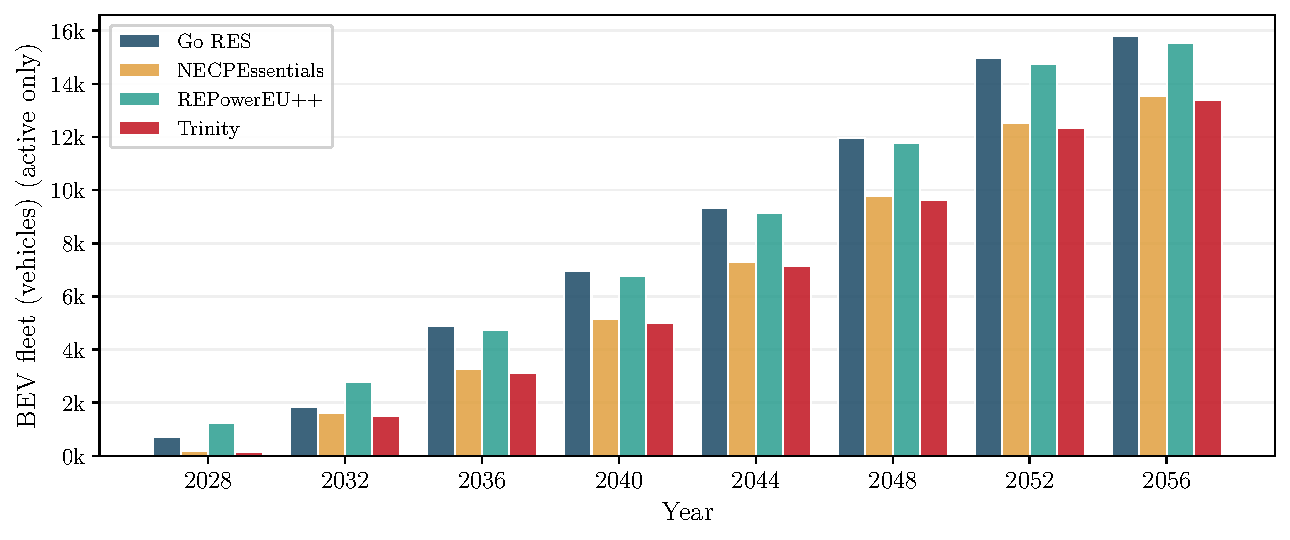
\includegraphics[width=0.9\linewidth]{graphics/paper_3/bev_fleet_growth_4scenarios.pdf}
    \caption{Battery-electric truck fleet growth across the four GENeSYS-MOD energy system scenarios along the Scandinavian-Mediterranean corridor. The scenarios group into two pairs: Go~RES and REPowerEU++ (higher adoption) and NECPEssentials and Trinity (lower adoption).}
    \label{fig:app_rq3_fleet_growth}
\end{figure}

\begin{figure}[H]
    \centering
    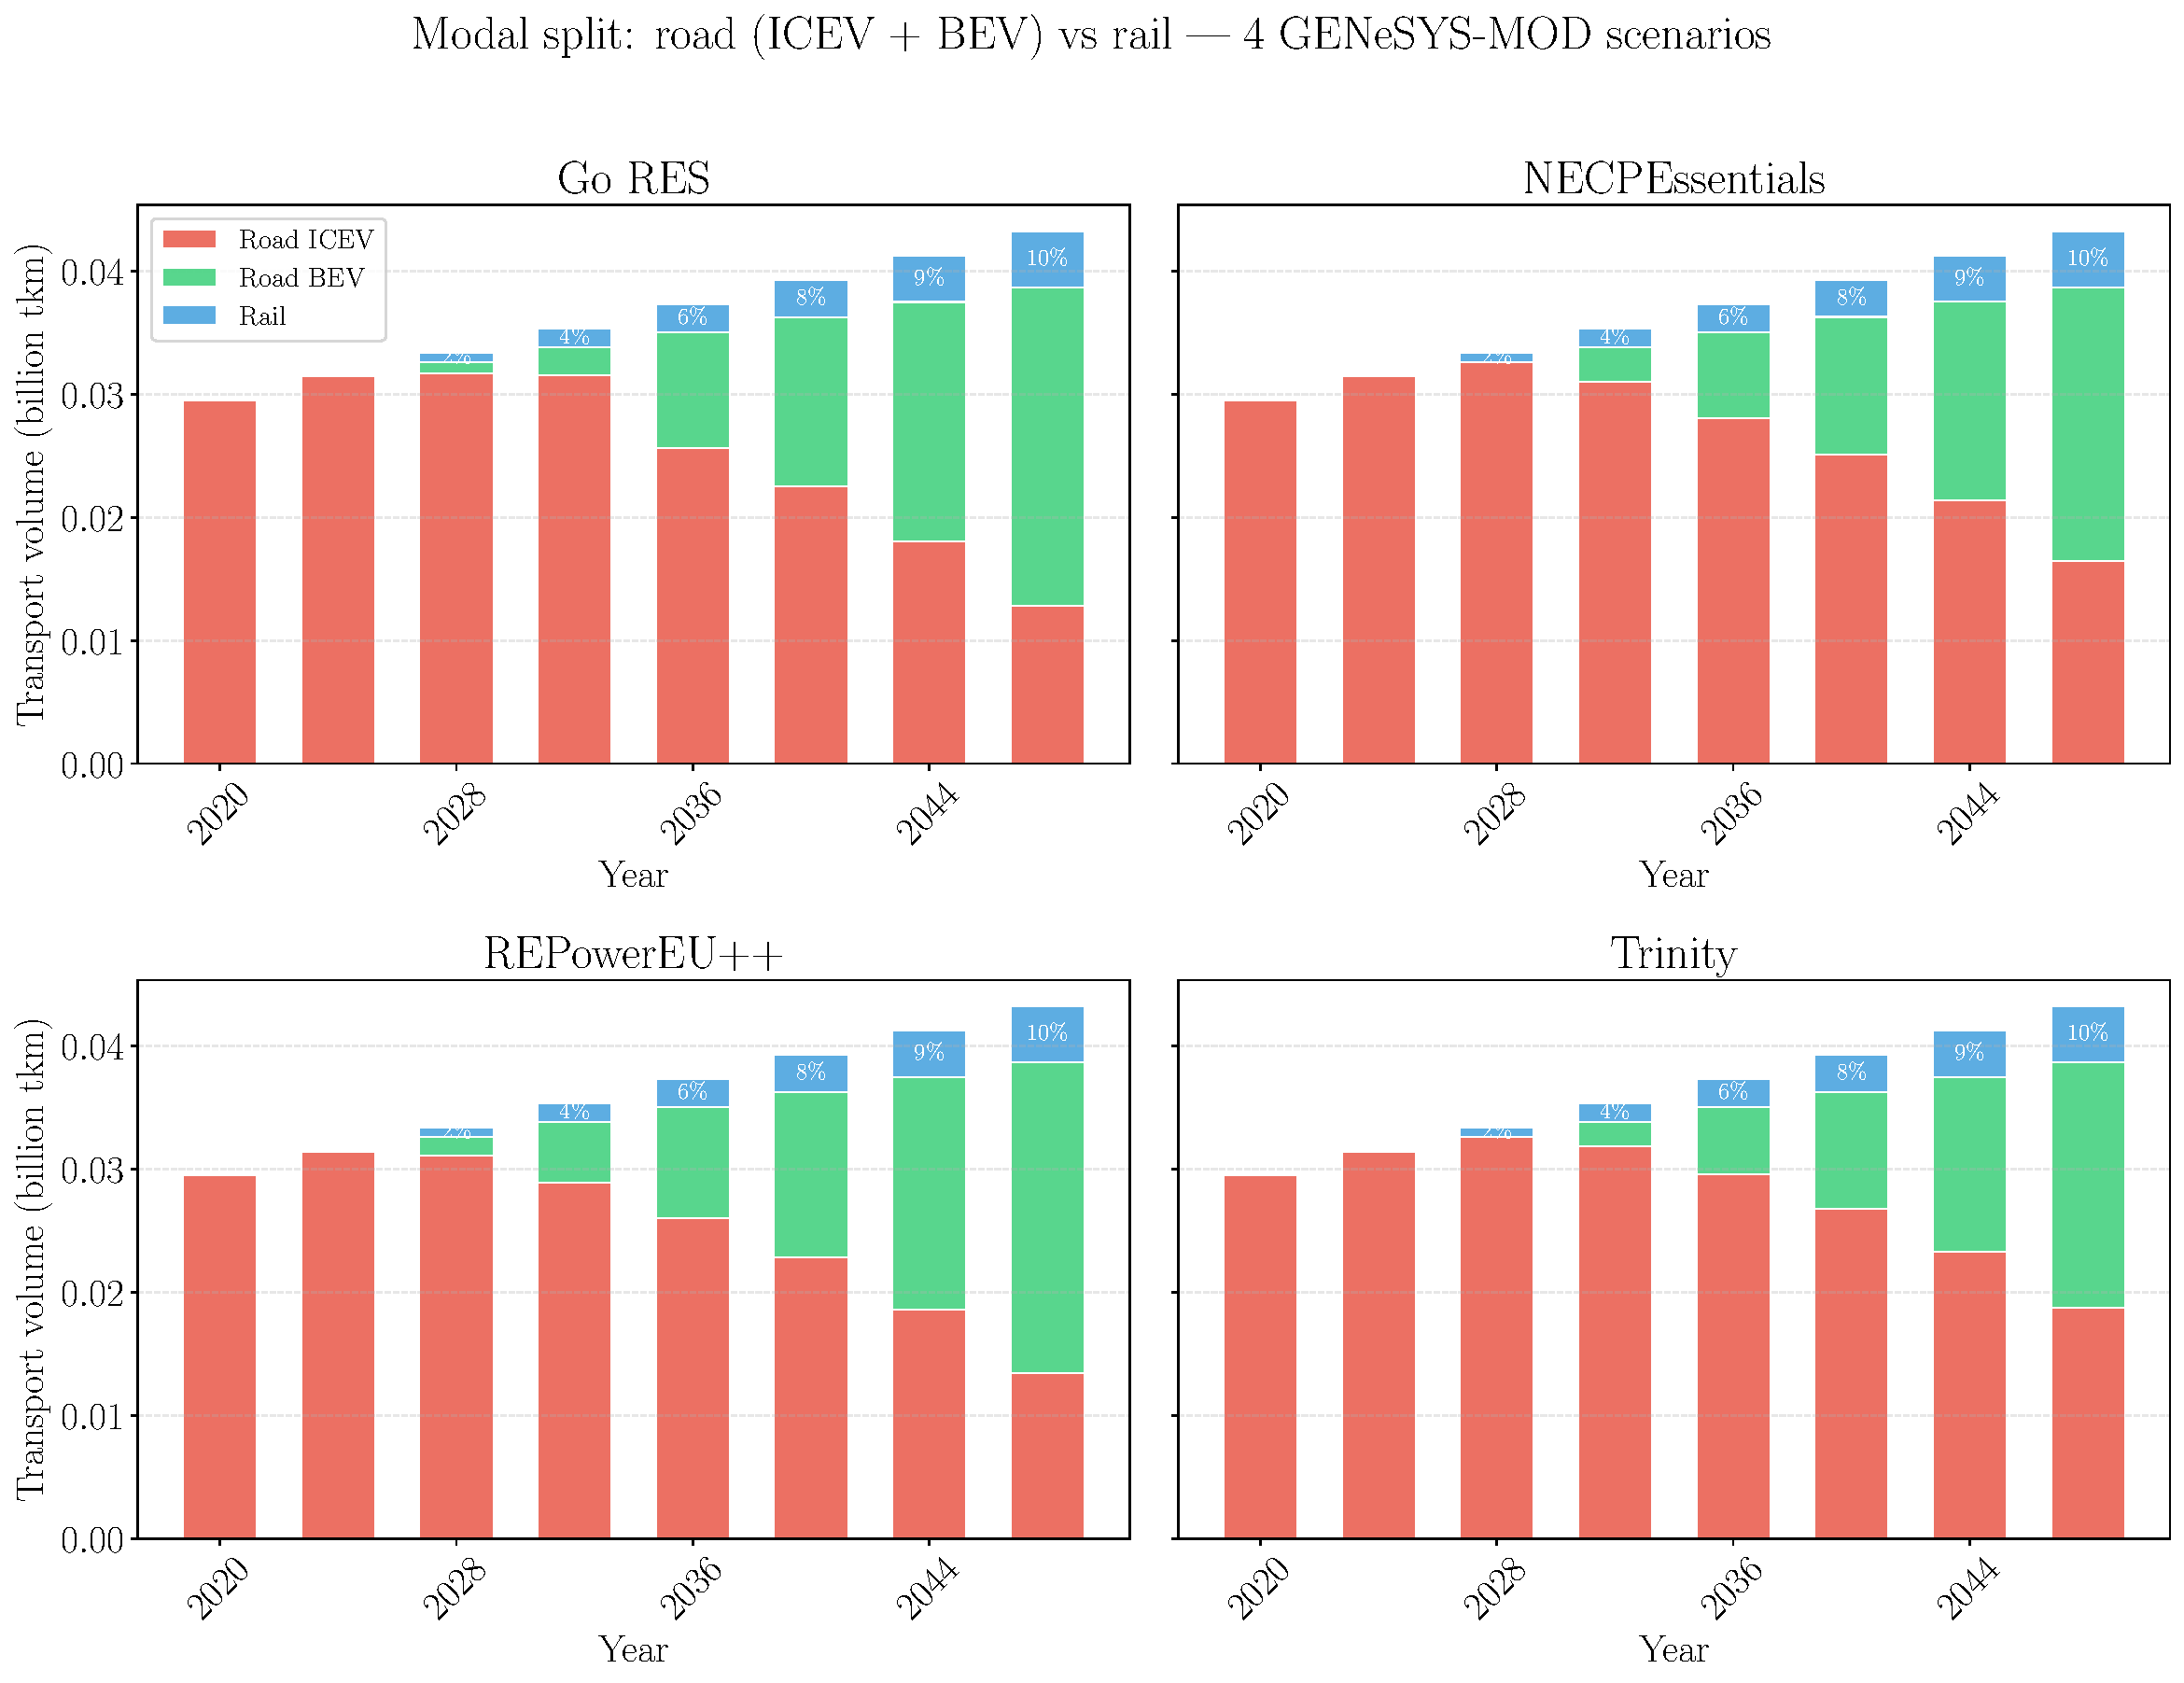
\includegraphics[width=\linewidth]{graphics/paper_3/modal_split_4scenarios_tkm.pdf}
    \caption{Modal split evolution for all four GENeSYS-MOD scenarios: transport volume (Mtkm) by mode and technology (road ICEV, road BET, and rail). The modal shift pattern is consistent across scenarios, with rail reaching approximately 10\% by 2048 in all cases.}
    \label{fig:app_rq3_modal_split}
\end{figure}

\begin{figure}[H]
    \centering
    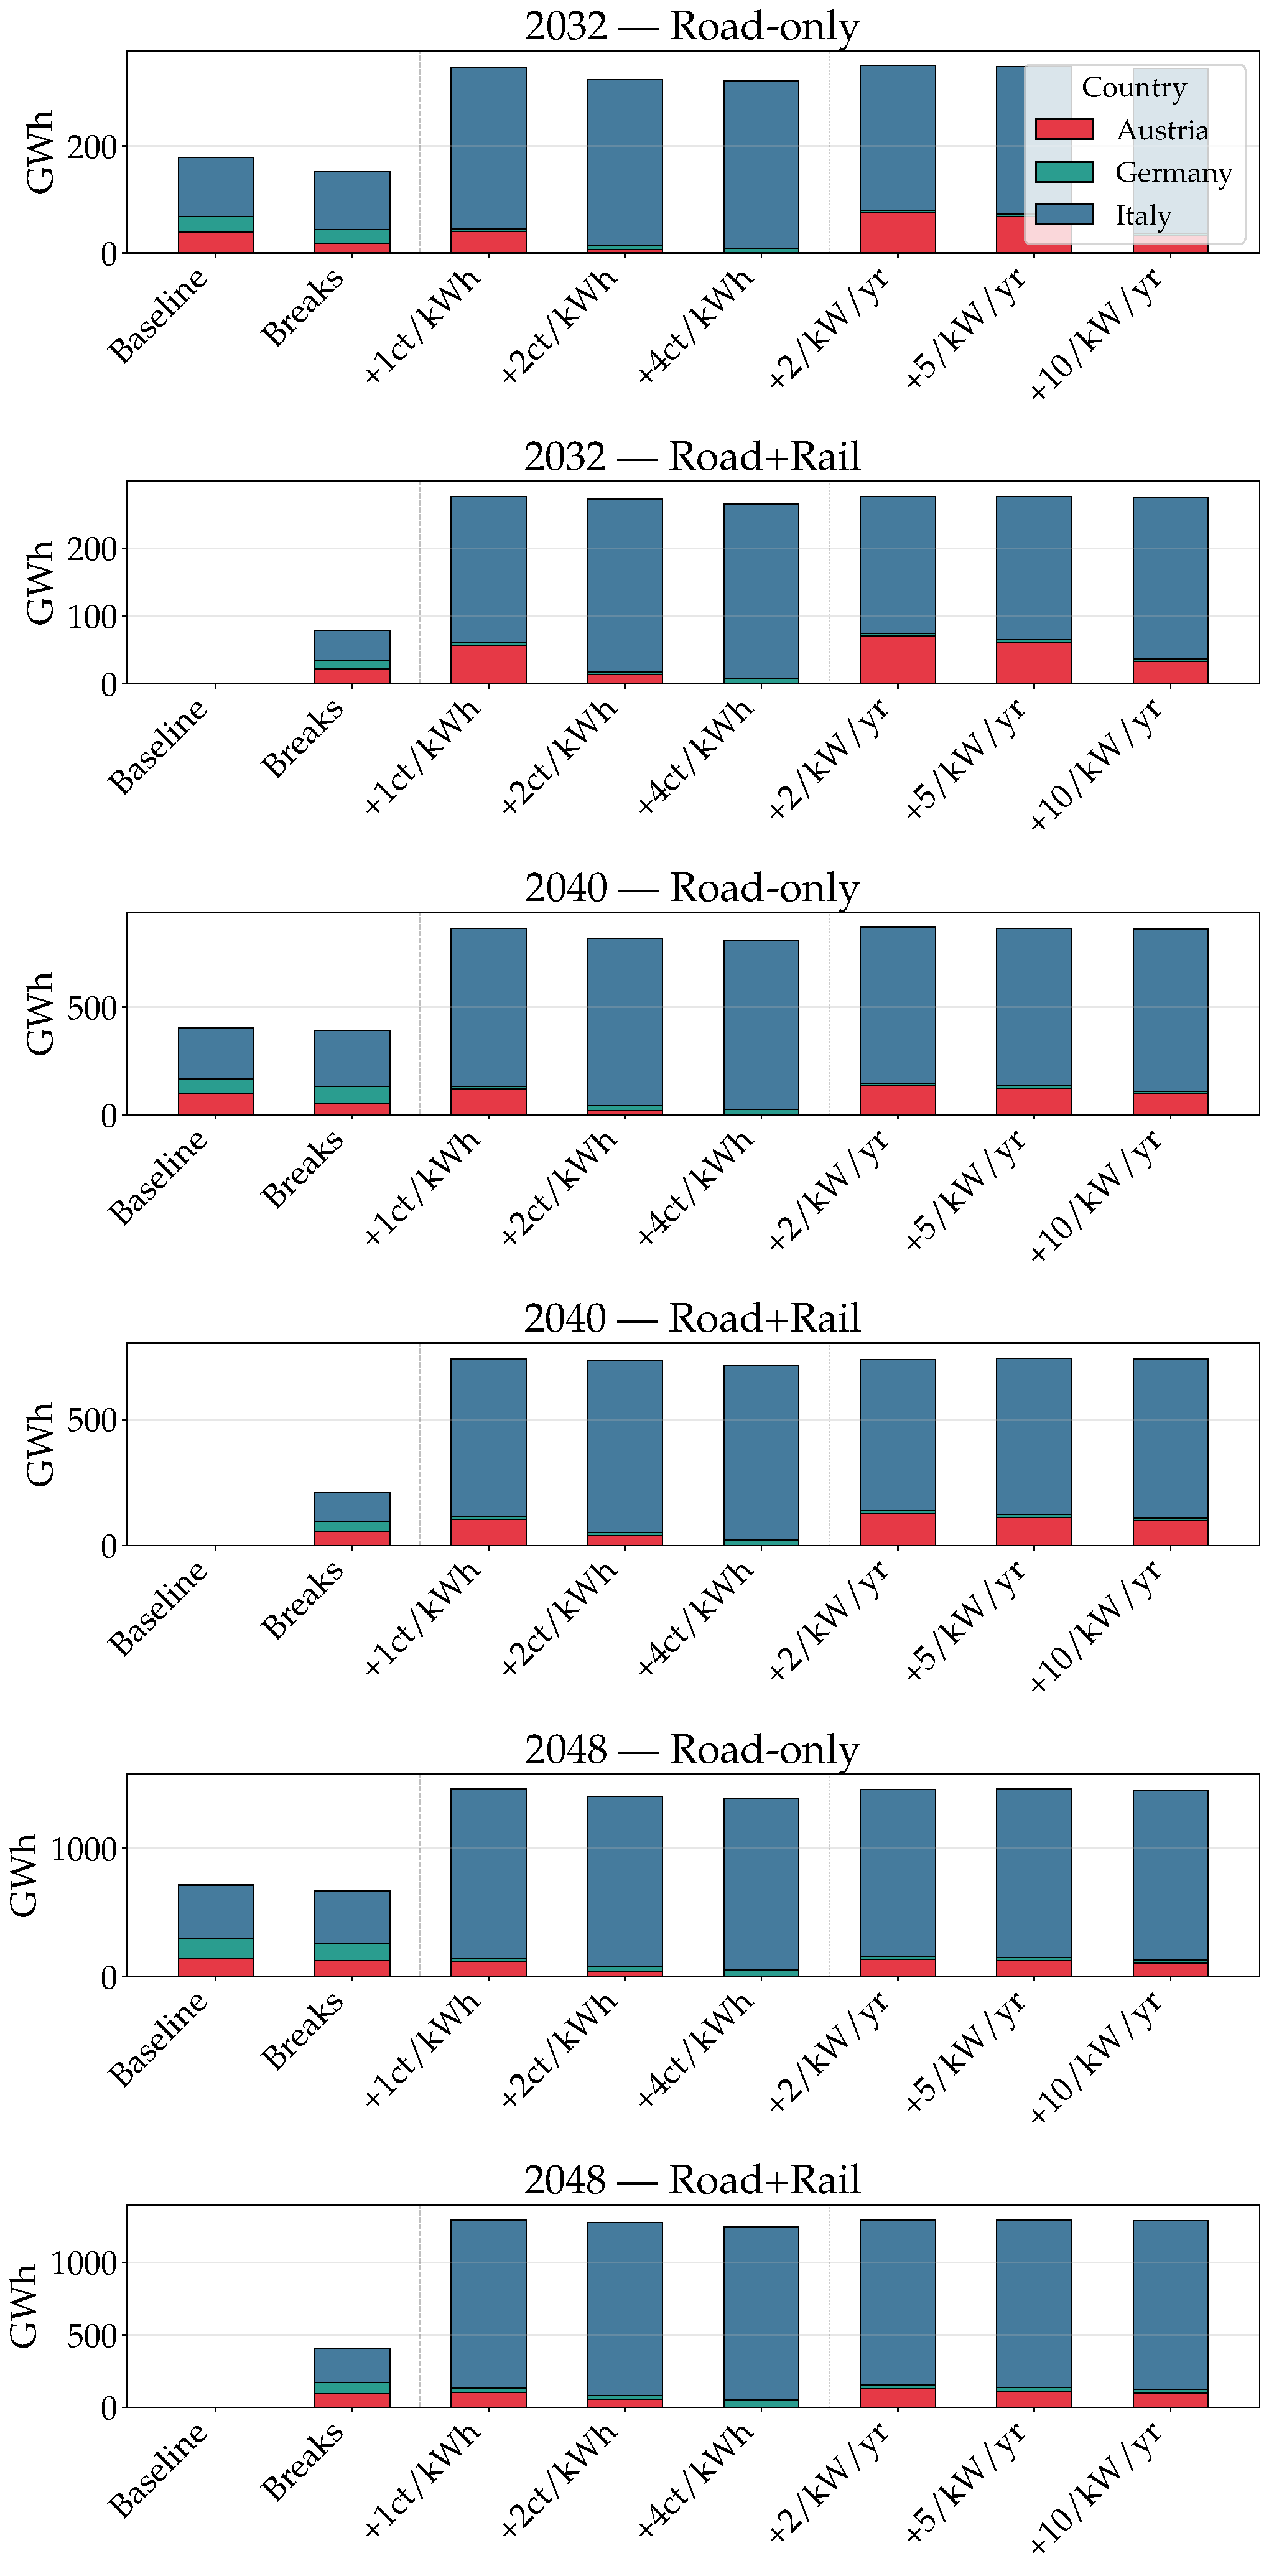
\includegraphics[width=0.55\linewidth]{graphics/paper_3/at_surcharge_border_charging_reallocation_3years.pdf}
    \caption{BET charging reallocation in the DE-AT-IT border region under Austrian electricity price and grid charge locational cost premiums for three time horizons (2032, 2040, 2048). Each panel shows stacked bars of charged energy (MWh) by country for reference scenarios (baseline, breaks constraint, fixed-fleet unconstrained) and graduated premium levels. Top rows: road-only; bottom rows: road with modal shift to rail.}
    \label{fig:app_rq3_surcharge_3years}
\end{figure}

\section{Computational details}\label{app:rq3_computational}

The model is implemented in Julia using JuMP~1.9 \citep{Lubin2023} and solved with Gurobi~12.0 \citep{gurobi}. Simulations are performed on an AMD Ryzen Threadripper 7980X (64 cores, 3.20~GHz base clock, 5.2~GHz boost) with 512~GB RAM.

The source code and input data are publicly available at: \url{https://github.com/antoniamgolab/iDesignRES_transcompmodel}.
